% Options for packages loaded elsewhere
\PassOptionsToPackage{unicode}{hyperref}
\PassOptionsToPackage{hyphens}{url}
\PassOptionsToPackage{dvipsnames,svgnames,x11names}{xcolor}
%
\documentclass[
  12pt,
]{article}
\usepackage{amsmath,amssymb}
\usepackage{lmodern}
\usepackage{iftex}
\ifPDFTeX
  \usepackage[T1]{fontenc}
  \usepackage[utf8]{inputenc}
  \usepackage{textcomp} % provide euro and other symbols
\else % if luatex or xetex
  \usepackage{unicode-math}
  \defaultfontfeatures{Scale=MatchLowercase}
  \defaultfontfeatures[\rmfamily]{Ligatures=TeX,Scale=1}
\fi
% Use upquote if available, for straight quotes in verbatim environments
\IfFileExists{upquote.sty}{\usepackage{upquote}}{}
\IfFileExists{microtype.sty}{% use microtype if available
  \usepackage[]{microtype}
  \UseMicrotypeSet[protrusion]{basicmath} % disable protrusion for tt fonts
}{}
\makeatletter
\@ifundefined{KOMAClassName}{% if non-KOMA class
  \IfFileExists{parskip.sty}{%
    \usepackage{parskip}
  }{% else
    \setlength{\parindent}{0pt}
    \setlength{\parskip}{6pt plus 2pt minus 1pt}}
}{% if KOMA class
  \KOMAoptions{parskip=half}}
\makeatother
\usepackage{xcolor}
\usepackage[margin=1in]{geometry}
\usepackage{graphicx}
\makeatletter
\def\maxwidth{\ifdim\Gin@nat@width>\linewidth\linewidth\else\Gin@nat@width\fi}
\def\maxheight{\ifdim\Gin@nat@height>\textheight\textheight\else\Gin@nat@height\fi}
\makeatother
% Scale images if necessary, so that they will not overflow the page
% margins by default, and it is still possible to overwrite the defaults
% using explicit options in \includegraphics[width, height, ...]{}
\setkeys{Gin}{width=\maxwidth,height=\maxheight,keepaspectratio}
% Set default figure placement to htbp
\makeatletter
\def\fps@figure{htbp}
\makeatother
\setlength{\emergencystretch}{3em} % prevent overfull lines
\providecommand{\tightlist}{%
  \setlength{\itemsep}{0pt}\setlength{\parskip}{0pt}}
\setcounter{secnumdepth}{5}
\newlength{\cslhangindent}
\setlength{\cslhangindent}{1.5em}
\newlength{\csllabelwidth}
\setlength{\csllabelwidth}{3em}
\newlength{\cslentryspacingunit} % times entry-spacing
\setlength{\cslentryspacingunit}{\parskip}
\newenvironment{CSLReferences}[2] % #1 hanging-ident, #2 entry spacing
 {% don't indent paragraphs
  \setlength{\parindent}{0pt}
  % turn on hanging indent if param 1 is 1
  \ifodd #1
  \let\oldpar\par
  \def\par{\hangindent=\cslhangindent\oldpar}
  \fi
  % set entry spacing
  \setlength{\parskip}{#2\cslentryspacingunit}
 }%
 {}
\usepackage{calc}
\newcommand{\CSLBlock}[1]{#1\hfill\break}
\newcommand{\CSLLeftMargin}[1]{\parbox[t]{\csllabelwidth}{#1}}
\newcommand{\CSLRightInline}[1]{\parbox[t]{\linewidth - \csllabelwidth}{#1}\break}
\newcommand{\CSLIndent}[1]{\hspace{\cslhangindent}#1}
\ifLuaTeX
\usepackage[bidi=basic]{babel}
\else
\usepackage[bidi=default]{babel}
\fi
\babelprovide[main,import]{ngerman}
% get rid of language-specific shorthands (see #6817):
\let\LanguageShortHands\languageshorthands
\def\languageshorthands#1{}

\usepackage[T1]{fontenc}
\usepackage[utf8]{inputenc}
\usepackage[scaled]{helvet}
\renewcommand\familydefault{\sfdefault}
\usepackage{setspace}

%math
\usepackage{mathtools, amssymb, amsthm} % imports amsmath
\usepackage{mathrsfs}
\usepackage{stmaryrd}

%captions
\usepackage[labelfont=bf]{caption}
\usepackage{floatrow}
\floatsetup[figure]{capposition=top}
\floatsetup[table]{capposition=top}

%acronyms
\usepackage[printonlyused,withpage]{acronym}

%für kable (tabellen) mit r erstellen
\usepackage{booktabs}
\usepackage{longtable}
\usepackage{array}
\usepackage{multirow}
\usepackage{wrapfig}
\usepackage{float}
%\floatplacement{figure}{H} % let the
%\floatplacement{table}{H}
\usepackage{colortbl}
\usepackage{pdflscape}
\usepackage{tabu}
\usepackage{threeparttable}
\usepackage{threeparttablex}
\usepackage[normalem]{ulem}
\usepackage{makecell}
\usepackage{xcolor}

\usepackage[german=quotes]{csquotes} %quotes

\usepackage[nottoc]{tocbibind}
\usepackage[toc,page]{appendix}


%geometry
\usepackage{geometry}\geometry{
 a4paper,
 left=20mm,
 top=20mm,
 right=20mm,
 bottom=20mm,
 }



%color
% \usepackage{sectsty}

% \definecolor{exampleuniversity}{RGB}{199, 16, 92}

% \colorlet{maincolor}{exampleuniversity}
% \colorlet{stringcolor}{green!60!black}
% \colorlet{commentcolor}{black!50}
% \colorlet{keywordcolor}{maincolor!80!black}

% \newcommand{\imagesuffix}{-color}

% \allsectionsfont{\color{maincolor}}

%for apendix
\usepackage{pdfpages}
%\usepackage{attachfile2}

\usepackage{afterpage}

\newcommand\blankpage{%
    \null
    \thispagestyle{empty}%
    \addtocounter{page}{-1}%
    \newpage}
\usepackage{booktabs}
\usepackage{longtable}
\usepackage{array}
\usepackage{multirow}
\usepackage{wrapfig}
\usepackage{float}
\usepackage{colortbl}
\usepackage{pdflscape}
\usepackage{tabu}
\usepackage{threeparttable}
\usepackage{threeparttablex}
\usepackage[normalem]{ulem}
\usepackage{makecell}
\usepackage{xcolor}
\ifLuaTeX
  \usepackage{selnolig}  % disable illegal ligatures
\fi
\IfFileExists{bookmark.sty}{\usepackage{bookmark}}{\usepackage{hyperref}}
\IfFileExists{xurl.sty}{\usepackage{xurl}}{} % add URL line breaks if available
\urlstyle{same} % disable monospaced font for URLs
\hypersetup{
  pdflang={de},
  colorlinks=true,
  linkcolor={Maroon},
  filecolor={Maroon},
  citecolor={Blue},
  urlcolor={blue},
  pdfcreator={LaTeX via pandoc}}

\author{}
\date{\vspace{-2.5em}}

\begin{document}

\pagenumbering{gobble}

\textbf{Seminararbeit von:}

\vskip0.25cm

NAME

MATRIKELNUMMER \hspace{1em}

ADRESSE

MAIL \hspace{1em}

TEL.NR.

HF: - X. Fachsemester \hspace{1em}

NF: - X. Fachsemester

\vskip0.5cm

\vfill

NAME\_KURS

Frau / Herr Prof.~Dr.~NACHNAME, VORNAME

Universität Kassel

Fachbereich 05 Geselschaftswissenschaften \pagebreak
\afterpage{\blankpage}

\setstretch{1}
\pagenumbering{roman}

\pagebreak
\afterpage{\blankpage}

\listoffigures

\pagebreak
\afterpage{\blankpage}

\listoftables

\pagebreak
\afterpage{\blankpage}

\tableofcontents

\pagebreak
\afterpage{\blankpage}

\setstretch{1.5}

\pagenumbering{gobble}

\hypertarget{abstract}{%
\section{Abstract}\label{abstract}}

\textbf{Zusammenfassung}

Die Kurzfassung sollte nicht länger als einige Absätze sein. Für die
deutsche Kurzfassung muss eine englische Version existieren, die eine
genaue Übersetzung der deutschen Fassung sein muss.

\textbf{Abstract}

The abstract should not be longer than some paragraphs. There must be an
English translation of the the German abstract, which has to be the
exact translation of the German version. \pagebreak

\pagenumbering{arabic}

\hypertarget{einleitung}{%
\section{Einleitung}\label{einleitung}}

Die Einleitung beinhaltet drei Elemente:

\begin{itemize}
\tightlist
\item
  Begründung der soziologischen Relevanz des Themas
\item
  Konkrete Forschungsfrage der Arbeit
\item
  Beschreibung des Fortgangs der Argumentation im weiteren Verlauf der
  Arbeit
\end{itemize}

\hypertarget{forschungsstand}{%
\section{Forschungsstand}\label{forschungsstand}}

Dieses Kapitel kann sich aus zwei Quellen speisen: Theorien und
bestehende empirische Befunde. Diese Zweiteilung kann durch Unterkapitel
manifestiert sein. Genauso gut können in einem gemeinsamen Kapitel zum
Forschungsstand theoretische Antworten und zugehörige empirische
Ergebnisse verwoben sein.

\hypertarget{theorien}{%
\subsection{Theorien}\label{theorien}}

Die ausgewhlten Theorien geben eine erste vorläufige Antwort auf die in
der Einleitung aufgeworfene Forschungsfrage. Dabei geht es in diesem
Kapitel darum, die Theorie insgesamt zu präsentieren und dann daraus
das, für die eigene Forschung verwendete, theoretische Modell zu
verdeutlichen. Wenn die Theorie nicht zu komplex ist, kann Sie auch in
Gänze empirisch untersucht werden. Aus den Theorien heraus müssen die
Mechanismen beschrieben werden, die den späteren Hypothesen zugrunde
liegen. Das bedeutet, die Erwartungen an z.B. eine bestimmte Wirkung
eines Sachverhalts muss begründet werden. Die Basis dieser Begründungen
kann durch eigene logische Überlegungen oder durch empirische Befunde
gelegt werden.

\hypertarget{empirische-befunde}{%
\subsection{Empirische Befunde}\label{empirische-befunde}}

In einem ersten Schritt sollte hier über Studien berichtet werden, die
ihren Fokus auf eine, der eigenen Forschung sehr nahe, Fragestellung
haben. Danach können Studien und ihre Ergebnisse einbezogen werden, die
sich mit Randaspekten der zu behandelnden Fragestellung beschäftigen.
Die empirischen Befunde sollen sich an der Forschungsfrage orientieren
und nicht am Forschungsfeld insgesamt. Die ausgewählten empirischen
Befunde sollen sich in den Hypothesen möglichst niederschlagen.

\hypertarget{hypothesen}{%
\section{Hypothesen}\label{hypothesen}}

Hypothesen beinhalten oft die Erwartungen über die Wirkungen eines
Sachverhalts auf einen anderen. Wir unterscheiden probabilistische
„Je\ldots desto``- Hypothesen von deterministischen „wenn \ldots{}
dann`` -- Sätzen. In einigen Fällen werden auch Unterschiede zwischen
Gruppen oder das Bestehen von Zusammenhängen zwischen gleichrangigen
Sachverhalten als Erwartungen formuliert.

\hypertarget{operationalisierung-und-datenbasis}{%
\section{Operationalisierung und
Datenbasis}\label{operationalisierung-und-datenbasis}}

Operationalisierung bezeichnet den Prozess, aus abstrakten Begriffen,
die aus den Hypothesen stammen, messbare Konstrukten in empirischen
Instrumenten abzuleiten. Die Konstrukte werden dann als Variablen oder
Items bezeichnet. Im Operationalisierungskapitel sollte es eine
Übersicht geben, die deutlich macht, welche Variable(n) welches
Konstrukt abbilden soll(en), welche Skalierung die Variablen aufweisen
und welche Wertelabels die einzelnen Skalenpunkte haben. Danach wird die
Datenbasis beschrieben. Dieser Aspekt umfasst Informationen dazu, wie
viele Elemente im Datensatz enthalten sind, wie die Grundgesamtheit
definiert wurde, wie die Stichprobenziehung erfolgte, wie die
Datenerhebung erfolgte (Erhebungsform, Zeitraum, regionale Verortung)
und unter Umständen, in welchem Format die Daten vorliegen (wide oder
long).

\hypertarget{empirische-analysen}{%
\section{Empirische Analysen}\label{empirische-analysen}}

\hypertarget{deskription}{%
\subsection{Deskription}\label{deskription}}

Im Kapitel zur Deskription werden dem Leser relevante Verteilungen in
geeigneter Form präsentiert. Relevante Verteilungen sind solche, die
zentrale Variablen aus den Hypothesen darstellen. Die Verteilung der
abhängigen Variable zählt in jedem Fall dazu. Geeignete Formen der
Präsentation von Verteilungen sind Grafiken, Tabellen und statistische
Maße zur Beschreibung von typischen Werten und dem Ausmaß an Streuung.
Welche Form man wählt, hängt vom Skalenniveau, der Anzahl der
Ausprägungen und davon ab, an welche Leserschaft sich der Text richtet.
Am wichtigsten ist für die Entscheidung der Darstellungsform die Antwort
auf die Frage, wie ein gutes und vollständiges Leseverständnis beim
Leser erreicht werden kann.

\hypertarget{tabelle}{%
\subsubsection{Tabelle}\label{tabelle}}

\begin{table}

\caption{\label{tab:unnamed-chunk-7}\label{tab:tab1}Lage und Streuungsmaße von Größe und Gewicht }
\centering
\begin{tabular}[t]{lrrrrrrr}
\toprule
  & n & mean & median & sd & min & max & range\\
\midrule
\cellcolor{gray!6}{Größe} & \cellcolor{gray!6}{59} & \cellcolor{gray!6}{174.02} & \cellcolor{gray!6}{180} & \cellcolor{gray!6}{35.53} & \cellcolor{gray!6}{66} & \cellcolor{gray!6}{234} & \cellcolor{gray!6}{168}\\
Gewicht & 59 & 97.31 & 79 & 169.46 & 15 & 1358 & 1343\\
\bottomrule
\end{tabular}
\end{table}

In der Tabelle \ref{tab:tab1} sind Lage und Streuungsmaße abgebildet.
Diese Tabelle wird autoomatisch in das Tabellenverzeichnis mit
aufgenommen.

Hier sind weitere Anpassungsmöglichkeiten für Tabellen:
\href{https://haozhu233.github.io/kableExtra/awesome_table_in_pdf.pdf}{Create
Awesome LaTeX Table with knitr::kable and kableExtra}

\hypertarget{abbildung}{%
\subsubsection{Abbildung}\label{abbildung}}

\begin{figure}

{\centering 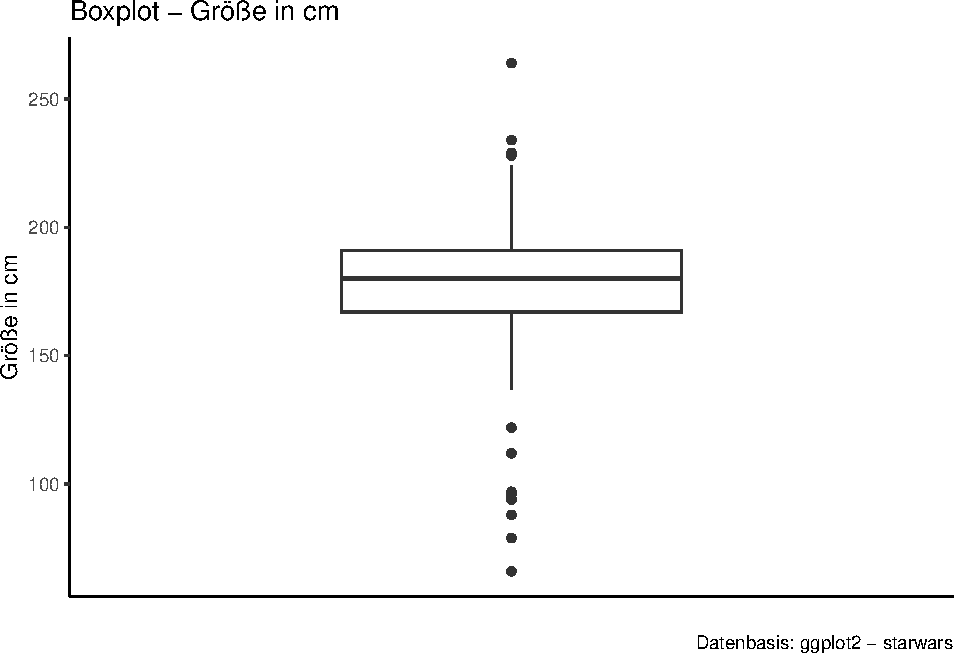
\includegraphics{thesis_files/figure-latex/unnamed-chunk-8-1} 

}

\caption{\label{fig:plt1}Boxplot - Größe in cm}\label{fig:unnamed-chunk-8}
\end{figure}

In der Abbildung \ref{fig:plt1} sieht man einen Boxplot zur Verteilung
der Körpergröße in cm. Auch diese Abbildung wird automatisch in das
Abbildungsverzeichnis aufgenommen.

\hypertarget{erkluxe4rungsmodelle}{%
\subsection{Erklärungsmodelle}\label{erkluxe4rungsmodelle}}

Im zweiten Teil der empirischen Analysen können Erklärungsmodelle
enthalten sein. Ausgewählt wird das Analyseverfahren zuerst nach dem
Skalenniveau der abhängigen Variable. Das Analyseverfahren muss diesem
entsprechen, dann ist es angemessen. Außerdem sollten die Modelle so
einfach wie möglich und so komplex wie nötig sein. Was nötig ist, ergibt
sich aus den Hypothesen und der Forschungsfrage. über die Hypothesen
hinausgehende Analysen und Interpretationen sind nur dann angebracht,
wenn sich damit eine neue Perspektive auf die Forschungsfrage ergibt.

\hypertarget{linear-regression-model-table}{%
\subsubsection{Linear Regression Model /
Table}\label{linear-regression-model-table}}

\begin{table}[!htbp] \centering 
  \caption{Regressionstabelle - OLS-Regressionen} 
  \label{tab:linreg1} 
\begin{tabular}{@{\extracolsep{5pt}}lcc} 
\\[-1.8ex]\hline 
\hline \\[-1.8ex] 
 & \multicolumn{2}{c}{\textit{Dependent variable:}} \\ 
\cline{2-3} 
\\[-1.8ex] & mass & height \\ 
\\[-1.8ex] & (1) & (2)\\ 
\hline \\[-1.8ex] 
 height & 0.639 &  \\ 
  & p = 0.313 &  \\ 
  mass &  & 0.028 \\ 
  &  & p = 0.313 \\ 
  Constant & $-$13.810 & 171.285$^{***}$ \\ 
  & p = 0.902 & p = 0.000 \\ 
 \hline \\[-1.8ex] 
Observations & 59 & 59 \\ 
R$^{2}$ & 0.018 & 0.018 \\ 
Adjusted R$^{2}$ & 0.001 & 0.001 \\ 
Residual Std. Error (df = 57) & 169.398 & 35.516 \\ 
F Statistic (df = 1; 57) & 1.040 & 1.040 \\ 
\hline 
\hline \\[-1.8ex] 
Notes: & \multicolumn{2}{l}{$^{*}$p$<$0.1; $^{**}$p$<$0.05; $^{***}$p$<$0.01} \\ 
 & \multicolumn{2}{l}{Abgetragen sind die nicht-standardisierten} \\ 
 & \multicolumn{2}{l}{Regressionskoeffizienten einer OLS- Regression.} \\ 
 & \multicolumn{2}{l}{Größe in cm} \\ 
 & \multicolumn{2}{l}{Gewicht in kg} \\ 
 & \multicolumn{2}{l}{Referenzkategorie:} \\ 
\end{tabular} 
\end{table}

In Tabelle \ref{tab:linreg1} ist eine Beispiel-Tabelle für eine lineare
Regression gerechnet.

\hypertarget{zusammenfassung-oder-fazit}{%
\section{Zusammenfassung oder Fazit}\label{zusammenfassung-oder-fazit}}

Schreiben Sie entweder eine Zusammenfassung oder ein Fazit. Eine
Zusammenfassung greift Aspekte, die im Analysekapitel bereits
ausführlich dargestellt sind kurz und prägnant auf und systematisiert
sie neu. Es dürfen keine neuen Überlegungen enthalten sein und es wird
in der Regel nicht aus der Literatur zitiert. Dagegen weitet ein Fazit
die Perspektive der Analyseergebnisse aus. Hier geht es darum, konkrete
Schlussfolgerungen aus den Ergebnissen zu ziehen, beispielsweise
Handlungsempfehlungen für spezifische Zielgruppen abzuleiten. Es ist
möglich, diese neuen Perspektiven auch wieder in die Fachdiskussion
einzubetten und mit Quellenverweisen zu arbeiten.

\pagebreak

\hypertarget{literaturverzeichnis}{%
\section{Literaturverzeichnis}\label{literaturverzeichnis}}

\hypertarget{refs}{}
\begin{CSLReferences}{0}{0}
\end{CSLReferences}

\pagebreak
\pagenumbering{gobble}

\hypertarget{anhang}{%
\section*{Anhang}\label{anhang}}
\addcontentsline{toc}{section}{Anhang}

\thispagestyle{empty}
\pagenumbering{gobble}

\end{document}
